\pdfminorversion=4
\documentclass[10pt, xcolor=dvipsnames]{beamer}
\setcounter{tocdepth}{1} % hide subsubsection in table of contents
\usetheme{Montpellier}
%\usetheme{CambridgeUS}
%\usecolortheme{lily}
\setbeamertemplate{footline}
{%
  \begin{beamercolorbox}[wd=\paperwidth,ht=0.5ex,dp=0ex,center]{footlinerule}
  \end{beamercolorbox}%
  \begin{beamercolorbox}[wd=\paperwidth,ht=0.6ex,dp=0ex,center]{empty}
  \end{beamercolorbox}%
  \leavevmode%
  \hbox{%
    \begin{beamercolorbox}[wd=.4\paperwidth,ht=2.25ex,dp=2ex,center]{author in head/foot}%
    \usebeamerfont{author in
head/foot}%
  \insertshortauthor\hspace{1em}(\insertshortinstitute)
  \end{beamercolorbox}%
  % \begin{beamercolorbox}[wd=.333333\paperwidth,ht=2.25ex,dp=2ex,center]{title in head/foot}%
  %   \usebeamerfont{title in head/foot}\insertshorttitle
  % \end{beamercolorbox}%
  \begin{beamercolorbox}[wd=.6\paperwidth,ht=2.25ex,dp=2ex,right]{date in head/foot}%
    \usebeamerfont{date in head/foot}\insertshortdate{}\hspace*{2em}
    \insertframenumber{} / \inserttotalframenumber\hspace*{2ex} 
  \end{beamercolorbox}}%
  \vskip0pt%
}%
\usepackage{appendixnumberbeamer}
\usepackage{graphicx}
\usepackage{tikz}
\usepackage{pgfplots}
\usepackage[american voltages]{circuitikz}
\usepackage{fourier}
\usepackage{braket}
\setbeamercovered{transparent}
%\usepackage{animate}
\usepackage{movie15}
\usetikzlibrary{decorations.pathmorphing, decorations.pathreplacing,shapes.multipart,angles,quotes,fadings,shapes.callouts,arrows}
% \title[Magnetic slowing of entrained high space density supersonic Lithium atoms]{Magnetic slower for entrained high space density supersonic cold Lithium atoms}
\title[Magnetic Field Oscillation]{Magnetic Field Oscillation in Adiabatic Slower System for Cold Atom Physics}
\author[Yu Lu, Nitish Mittal, Xingyao Wang]{Yu Lu, Graduate student, Dept. of Physics \\  Nitish Mittal, Graduate student, Colllege of Pharmacy \\ Xingyao Wang, Graduate student, CSEM}

\institute{University of Texas at Austin}
\date{December 1st, 2016}
\setbeamercovered{invisible}
\begin{document}
% --------------------------------------------- title page -----------------------------------------
\begin{frame}
  \titlepage
\end{frame}


\section[Introduction]{Adiabatic slower in Cold Atom Physics}

\begin{frame}
  \frametitle{Adiabatic slower and Field Oscillation}
  \begin{columns}
    \column{0.5\textwidth}
    \begin{figure}
      \graphicspath{{./images/}}
      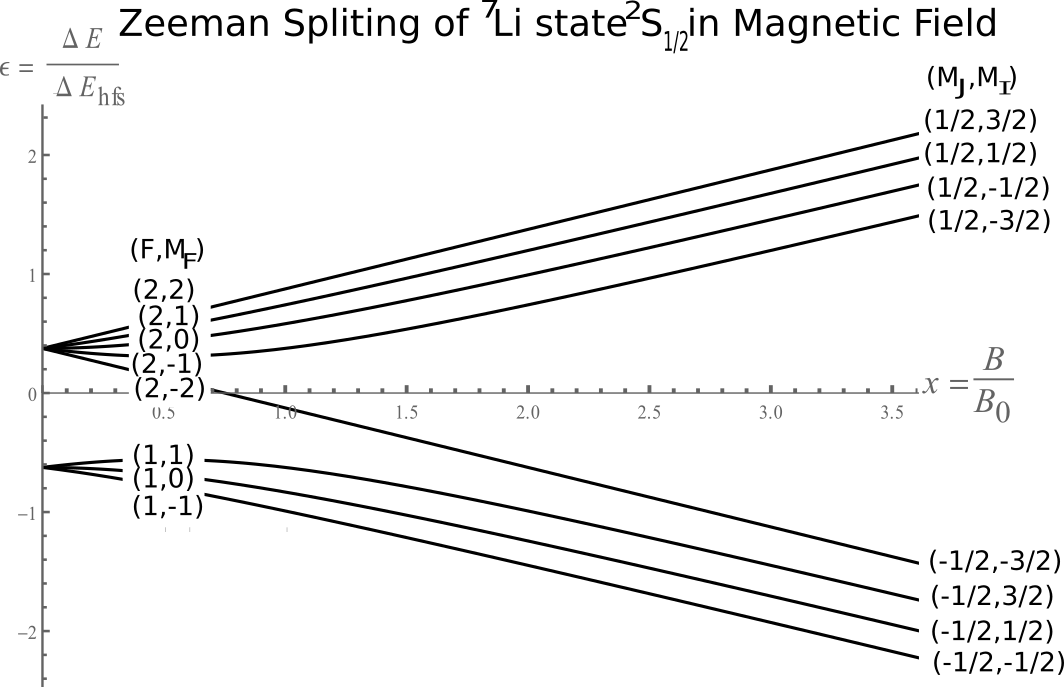
\includegraphics[width=\textwidth, height=0.6\textheight]{ZeemanSplit}
    \end{figure}
    \tiny{http://demonstrations.wolfram.com/BreitRabiDiagram/}\\
    
    \column{0.4\textwidth}
    \begin{tikzpicture}[x=2mm,y=2mm, overlay]
      % ----------------------------------1---------------------------------
      % draw atoms low
      \onslide<3>{
        \begin{scope}[scale=0.5,shift={(0,-20)}] 
          \shadedraw[ball color = red!90] (5,0) circle (1);
          \shadedraw[ball color = red!90] (4.5,1.5) circle (1);
          \shadedraw[ball color = red!90] (6,1.5) circle (1);
          \shadedraw[ball color = red!90] (7,0.5) circle (1);
          \shadedraw[ball color = red!90] (5,3) circle (1);
          \shadedraw[ball color = red!90] (7,3) circle (1);
          \draw[->, line width=2pt, blue]  (7,2) -- (15,2) node[below]{$V_{atom}$};
          \draw[->, line width=2pt, red]  (2,7) -- (6,7) node[above]{$V_{trap}$};
        \end{scope}
      }
      \onslide<2-3>{
        \begin{scope}[shift={(-6,-16)}, line width=1,color=red!50]
          \draw[out=0, in=180] (1,5) to (2,5);
          \draw[out=60] (2,5) parabola bend (5,15)(6,14);
          \draw (6,14) to (8,6);
          \draw(8,6) parabola bend (9,5)(10,6);
          \draw[out=0](10,6) parabola bend  (14,15)(15,14);
          \draw[out=300,in=180] (15,14) to  (19,5);
        \end{scope}
      }
      

      
      \onslide<4>{
        \begin{scope}[shift={(4,-10)}]
          \begin{scope}[scale=0.5]
            \shadedraw[ball color = green!60] (5,0) circle (1);
            \shadedraw[ball color = green!60] (4.5,1.5) circle (1);
            \shadedraw[ball color = green!60] (6,1.5) circle (1);
            \shadedraw[ball color = green!60] (7,0.5) circle (1);
            \shadedraw[ball color = green!60] (5,3) circle (1);
            \shadedraw[ball color = green!60] (7,3) circle (1);
            \draw[->, line width=2pt, blue]  (7,2) -- (15,2) node[below]{$V_{atom}$};
            \draw[->, line width=2pt, red]  (2,7) -- (6,7) node[above]{$V_{trap}$};
          \end{scope}
          \begin{scope}[shift={(-6,-6)}, line width=1,color=red!50]
            \draw[out=0, in=180] (1,5) to (2,5);
            \draw[out=60] (2,5) parabola bend (5,15)(6,14);
            \draw (6,14) to (8,6);
            \draw(8,6) parabola bend (9,5)(10,6);
            \draw[out=0](10,6) parabola bend  (14,15)(15,14);
            \draw[out=300,in=180] (15,14) to  (19,5);
          \end{scope}
        \end{scope}
      }

      \onslide<5>{
        \begin{scope}[shift={(8,-10)}]
          \begin{scope}[scale=0.5]
            \shadedraw[ball color = blue!60] (5,0) circle (1);
            \shadedraw[ball color = blue!60] (4.5,1.5) circle (1);
            \shadedraw[ball color = blue!60] (6,1.5) circle (1);
            \shadedraw[ball color = blue!60] (7,0.5) circle (1);
            \shadedraw[ball color = blue!60] (5,3) circle (1);
            \shadedraw[ball color = blue!60] (7,3) circle (1);
            \draw[->, line width=2pt, blue]  (7,2) -- (15,2) node[below]{$V_{atom}$};
            \draw[->, line width=2pt, red]  (2,7) -- (6,7) node[above]{$V_{trap}$};
          \end{scope}
          \begin{scope}[shift={(-6,-6)}, line width=1,color=red!50]
            \draw[out=0, in=180] (1,5) to (2,5);
            \draw[out=60] (2,5) parabola bend (5,15)(6,14);
            \draw (6,14) to (8,6);
            \draw(8,6) parabola bend (9,5)(10,6);
            \draw[out=0](10,6) parabola bend  (14,15)(15,14);
            \draw[out=300,in=180] (15,14) to  (19,5);
          \end{scope}
        \end{scope}
      }

      \node<2-> at (5,5){
        \graphicspath{{./images/}}
        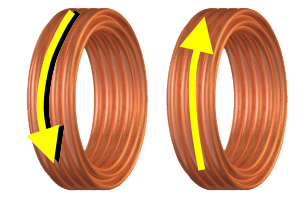
\includegraphics[width=0.5\textwidth]{AntiHelmhotzSym}
      };
      \node<2-> at (5,12)[fill=blue!20] {Anti-Helmholtz Coil};
    \end{tikzpicture}
  
  \end{columns}
  \onslide<2->{
  \vspace{2mm}
  \tiny{E. Narevicius and M. G. Raizen. Chem. Rev. 112, 4879 (2012)}
  }
\end{frame}

\begin{frame}
  \frametitle{Field switching}

  \begin{tikzpicture}[scale=0.25]
    \def \holedia {4};
    \def \boxlen {6};
    \def \boxwid {4};
    % axis and direction
    \onslide<1->{
      \draw[->,blue,line width=1pt]  (2,3) -- ++(2,0) node[right] {$\vec{V}_{atoms}$};
      \draw[dashed,line width=2] (1,2) -- ++(30,0)node[right,text width=1cm]{\small{Symmetry\\Axis}};
      
      % Boxes and circles
      \foreach \x in {0,6,...,24}{
        \draw[dashed,orange,line width=1.5] (\x,\holedia) rectangle ++(\boxlen,\boxwid);
        \foreach \y in {0.5,1.5,...,3.5}
        \foreach \z in {0.5,1.5, ..., 5.5} \draw[line width=0.8] (\x+\z, \holedia+\y) circle(0.5);
      }
      % trap 1
      \foreach \x in {4.5,5.5,12.5,13.5,14.5,15.5}
      \foreach \y in {0.5,1.5,...,3.5} \fill[blue] (\x,\y+\holedia) circle (0.5);
      \draw[blue,line width=2]
      (5.5, 7.5) ..controls +(up:2) and +(up:2).. (12.5,7.5);
      \draw[blue,line width=2]
      (4.5, 7.5) --  ++(0,2.5)
      (4.5, 9.5)[<-] -- ++(0,2);
      \draw[blue,line width=2]
      (15.5,10) -- ++(0,2)
      (15.5,7.5)[->] -- ++(0,2.5);
      
      
      % trap 2
      \foreach \x in {4.5,5.5,12.5,13.5,14.5,15.5}
      \foreach \y in {0.5,1.5,...,3.5} \fill[red] (\x+6,\y+\holedia) circle (0.5);
      \draw[red,line width=2]
      (11.5, 7.5) ..controls +(up:2) and +(up:2).. (18.5,7.5);
      \draw[red,line width=2]
      (10.5, 7.5) --  ++(0,2.5)
      (10.5, 9.5)[<-] -- ++(0,2);
      \draw[red,line width=2]
      (21.5,10)[->] -- ++(0,2)
      (21.5,7.5) -- ++(0,2.5);
      
      
      
      % trap 3
      \foreach \x in {4.5,5.5,12.5,13.5,14.5,15.5}
      \foreach \y in {0.5,1.5,...,3.5} \fill[green] (\x+12,\y+\holedia) circle (0.5);
      \draw[green,line width=2]
      (17.5, 7.5) ..controls +(up:2) and +(up:2).. (24.5,7.5);
      \draw[green,line width=2]
      (16.5, 7.5) --  ++(0,2.5)
      (16.5, 9.5)[<-] -- ++(0,2);
      \draw[green,line width=2]
      (27.5,10)[->] -- ++(0,2)
      (27.5,7.5) -- ++(0,2.5);
    }
    \onslide<2->{
      % Axis
      \draw[->,line width=1pt] (0,-3.3)-- ++(35,0) node[below]{Position};
      \draw[->,line width=1pt] (0,-3.3)-- ++(0,5) node[midway,left]{Potential};
      \draw[->,black, line width=1pt] (0,-10) --++ (35,0) node[right]{Time};
      \draw[->,black, line width=1pt] (0,-10) --++ (0,5) node[midway,left]{Current};
    }
    \onslide<3->{
      % 1st cycle
      % trap 1 field
      \begin{scope}[shift={(0,-5)},yscale=0.4,blue, line width=1]
        \draw[out=0,in=180] (2,5) to (5,9);
        \draw[out=0,in=180] (5,9) to (9,5);
        \draw[out=0](9,5) parabola bend  (14,15)(15,14);
        \draw[out=300,in=180] (15,14) to  (19,5);
      \end{scope}
      % trap 1 current
      \draw[scale=4,domain=0:0.66*pi,smooth,samples=20,yshift=-71,xshift=10,blue, line width=1pt] plot (\x, {sin(1.5*\x r)});
      \draw[decorate,decoration={brace,mirror,amplitude=0.2cm},blue,line width=1pt] (1.8,-10.2) -- ++(4,0)node[midway,below=0.1cm] {\tiny{$T_1/4$}};
    }
    \onslide<4->{
      % trap 2 field
      \begin{scope}[shift={(6,-5)},yscale=0.4,red, line width=1]
        \draw[out=0,in=180] (2,5) to (5,9);
        \draw[out=0,in=180] (5,9) to (9,5);
        \draw[out=0](9,5) parabola bend  (14,15)(15,14);
        \draw[out=300,in=180] (15,14) to  (19,5);
      \end{scope}
      % trap 2 current
      \draw[scale=4,domain=0:pi,smooth,samples=20,yshift=-71,xshift=40,red, line width=1pt] plot (\x, {sin(\x r)});
      \draw[decorate,decoration={brace,mirror,amplitude=0.2cm},red,line width=1pt] (5.8,-10.2) -- ++(6,0)node[midway,below=0.1cm] {\tiny{$T_2/4$}};
      % 3rd cycle
    }
    \onslide<5->{
      % trap 3 field
      \begin{scope}[shift={(12,-5)},yscale=0.4,green, line width=1]
        \draw[out=0,in=180] (2,5) to (5,9);
        \draw[out=0,in=180] (5,9) to (9,5);
        \draw[out=0](9,5) parabola bend  (14,15)(15,14);
        \draw[out=300,in=180] (15,14) to  (19,5);
      \end{scope}
      % trap 3 current
      \draw[scale=4,domain=0:1.66*pi,smooth,samples=20,yshift=-71,xshift=85,green, line width=1pt] plot (\x, {sin(0.6*\x r)});
      \draw[decorate,decoration={brace,mirror,amplitude=0.2cm},green,line width=1pt] (11.9,-10.2) -- ++(10,0)node[midway,below=0.1cm] {\tiny{$T_3/4$}};
    }
  \end{tikzpicture}
\end{frame}

\section{Objective}
\begin{frame}
  \frametitle{Objective}
  Study the oscillation of magnetics field minimium during the transition
\end{frame}

\section{Method}
\begin{frame}
  \frametitle{Method}
  Programming languages: C++, Python, Shell \\[3mm]
  \begin{itemize}
  \item Construct coil geometry and loacation
  \item Generate time dependent current in coils
  \item Loop Through time for certain periods.
  \item At each time point, loop through traps and position, calculate field distribution.
  \item Search for field minimium point and return position and value
  \item Save data file into csv file
  \item Call Python3 through Makefile to generate and save plots.
  \item Call Shell through Makefile to combine plots into gif. 
  \end{itemize}
\end{frame}

\section{Result}
\begin{frame}
  
\begin{frame}

\end{document}